
\section{Sentiment Representation Structures}
\subsection{Ekman's Six Basic Emotions}

There is no universally accepted model for representing emotion, but a standard for classifying emotions in a categorical model is using Ekmans six basic emotions \cite{Ekman}. These are identified as Anger, Disgust, Fear, Happiness, Sadness and Surprise. Being able to use these fundamental emotions to represent the sentiment of a text allows for more insight into the emotions around it. Since there are only six discrete classes in which emotions can be placed, this can be argued to be very subjective when classifying however \cite{emoBank}.

\subsection{Valence}
A very common way to classify phrases and sentences in sentiment analysis is to analyse the valence of the text \cite{frijda1986emotions}.

The valence of a piece of text is how positive or negative the emotion behind it is. An example of a sentence with a high valence would be "I am feeling very happy, I'm having a great day!", compared to a low valence, "I am having a terrible day, everything is going wrong". 

As this is a dimensional model, where values chosen could be hypothetically infinite this can represent a wider range than just six classes such as Ekmans emotions, however only measuring the positivity or negativity of a text does not provide much insight into it.
Using valence in a machine learning context is very useful though, as commonly the valence values can be put into discrete binary classes, positive or negative, and is a good base to start from.

\subsection{Circumplex Model}
The Circumplex Model is a 2 dimensional way of representing emotions, using a Valence or Pleasure measure and an Arousal or Activation measure \cite{modelOfAffect}.

\begin{figure}[h]
\caption{Graph of the Circumplex model with the $x$ axis representing the Valence and the $y$ axis representing the Arousal}
\centering
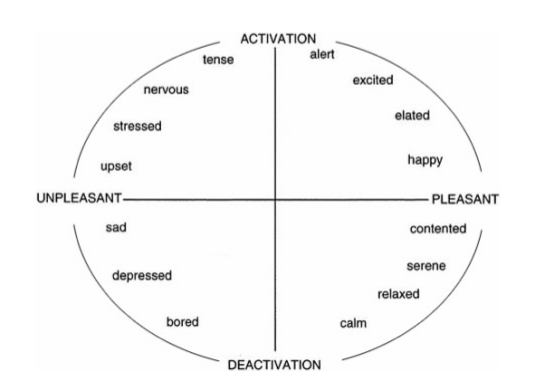
\includegraphics[scale=0.4]{./LitReview/images/circumplex.png}
\end{figure}

However there have been issues raised with this model \cite{circumplexIssues},  with concerns that only having two dimensions is not enough to be able to properly classify a human emotion.

\subsection{Valence Arousal Dominance Structure}
Building on the Circumplex Model, combating some of the issues raised with it comes the Valence-Arousal-Dominance Structure.
Known also as the as the Pleasure-Arousal-Dominance, the Valence-Arousal-Dominance structure (referred hereafter as VAD) introduced in 1974 \cite{PAD} \cite{VAD} provides a 3D representation for emotions, with each variable being defined as follows:
\begin{itemize}
    \item Valence- How positive or negative the statement is.
    \item Arousal- Degree of calmness or excitement, the energy of the statement. 
    \item Dominance- Degree of control over a situation.
\end{itemize}

Using VAD values allow for easy representation into the Ekman six basic emotions, as although there is no standard on the exact VAD values to use for each emotion, the primary dataset that will be used references values given by Russell and Mehrabian \cite{VADMapping}, which are shown below:

\begin{center}
\begin{tabular}{ |c|c|c|c|c|c|c| } 
 \hline
  & Anger & Disgust & Fear & Happiness & Sadness & Surprise \\ 
 \hline                        
 Valence & -0.51 & -0.6 & -0.64 & 0.81 & -0.63 & 0.4\\ 
 Arousal & 0.59 & 0.35 & 0.6 & 0.51 & -0.27 & 0.67\\ 
 Dominance & 0.25 & 0.11 & -0.43 & 0.46 & -0.33 & -0.13\\ 
 \hline
\end{tabular}
\end{center}

\begin{figure}[h]
\caption{Graph showing the affective space spanned by the three VAD dimensions showing Ekmans six basic emotions \cite{VADMapping}}
\centering
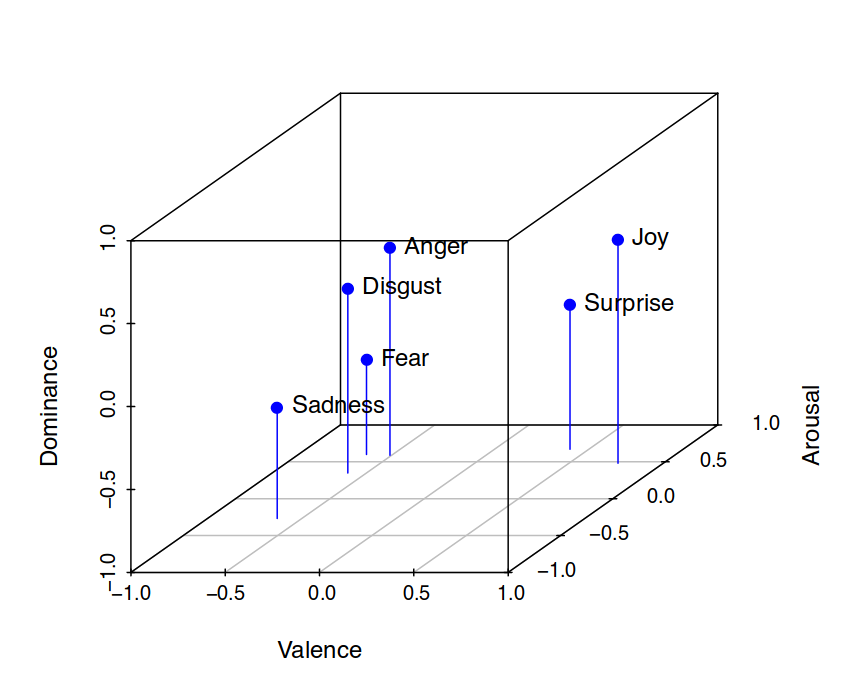
\includegraphics[scale=0.2]{./LitReview/images/VAD_Ekman.png}
\label{ekmans:graph}
\end{figure}

Using the VAD structure to represent sentiment in this project was ideal, as it allows for much more description of emotion in text \cite{emotionPerspective}, and having numeric values means its easy to work with.